% Datei: chapters/05_atommodelle/05_grenzen_klassischer_atommodelle.tex

\subsection{Grenzen der klassischen Atommodelle}
\index{Klassische Atommodelle}
\index{Atommodell!Grenzen}
\index{Bohrsches Atommodell}
\index{Sommerfeldsches Atommodell}
\index{Quantenmechanik}
\index{Elektronenhülle}
\index{Wellenfunktion}
\index{Aufenthaltswahrscheinlichkeit}

Die Atommodelle von Thomson, Rutherford, Bohr und Sommerfeld waren wichtige
Schritte auf dem Weg zum modernen Atomverständnis. Jedes dieser Modelle löste
ein bestimmtes Problem, erzeugte aber zugleich neue Fragen. Genau darin liegt
ihre historische Bedeutung: Sie zeigten immer deutlicher, dass das Atom nicht
mehr vollständig mit klassischer Physik beschrieben werden konnte.

Das thomsonsche Modell machte das Elektron erstmals zu einem Bestandteil des
Atoms. Es erklärte die elektrische Neutralität des Atoms durch eine positive
Ladungsmasse, in die negativ geladene Elektronen eingebettet waren. Sein
grundlegendes Problem bestand jedoch darin, dass es keinen Atomkern kannte.
Die Ergebnisse des Goldfolienexperiments waren mit diesem Modell nicht
vereinbar.

Das rutherfordsche Kernmodell beseitigte diese Schwäche. Es zeigte, dass die
positive Ladung und fast die gesamte Masse des Atoms in einem winzigen Kern
konzentriert sind. Die Elektronen befinden sich in der Hülle. Damit entstand
das Bild eines Atoms aus Kern und Elektronenhülle.

Dieses Modell hatte jedoch ein schweres Stabilitätsproblem. Ein Elektron, das
sich klassisch auf einer Bahn um den positiv geladenen Kern bewegt, ist
beschleunigt. Nach der klassischen Elektrodynamik müsste es elektromagnetische
Strahlung aussenden, Energie verlieren und schließlich in den Kern stürzen.
Ein klassisches Rutherford-Atom wäre daher nicht dauerhaft stabil.

Bohr löste dieses Problem durch die Annahme stationärer Bahnen. Elektronen
durften sich nur auf bestimmten erlaubten Bahnen bewegen und dort keine Energie
abstrahlen. Übergänge zwischen diesen Bahnen führten zur Aussendung oder
Aufnahme von Photonen:

\[
\Delta E = h f
\]

Damit konnte das Wasserstoffspektrum erfolgreich erklärt werden. Dennoch blieb
das bohrsche Modell in einem entscheidenden Punkt widersprüchlich: Es verwendete
weiterhin klassische Kreisbahnen, verbot aber gleichzeitig die klassische
Strahlung auf diesen Bahnen. Die Quantisierung wurde als zusätzliche Regel
eingeführt, aber noch nicht aus einer tieferen Theorie abgeleitet.

Sommerfeld verbesserte das bohrsche Modell durch elliptische Bahnen,
zusätzliche Quantenzahlen und relativistische Korrekturen. Damit konnten
bestimmte Feinheiten der Spektren besser beschrieben werden. Trotzdem blieb
auch dieses Modell ein Bahnmodell. Es stellte sich das Elektron weiterhin als
kleines Teilchen vor, das sich auf einer bestimmten Bahn um den Kern bewegt.

Genau diese Vorstellung wurde später aufgegeben. In der modernen Quantenmechanik
besitzt ein Elektron im Atom keine klassische Bahn mehr. Es wird nicht durch
einen festen Ort und eine feste Umlaufbahn beschrieben, sondern durch einen
quantenmechanischen Zustand. Dieser Zustand liefert Wahrscheinlichkeiten dafür,
wo das Elektron bei einer Messung gefunden werden kann.

An die Stelle der Elektronenbahn tritt daher die Wellenfunktion. Sie enthält
die Information über den Zustand des Elektrons. Aus ihr erhält man die
Aufenthaltswahrscheinlichkeit des Elektrons im Atom. Die Elektronenhülle ist
damit kein System kleiner Planetenbahnen, sondern eine räumliche
Wahrscheinlichkeitsverteilung.
\FloatBarrier
\begin{figure}[H]
	\centering
	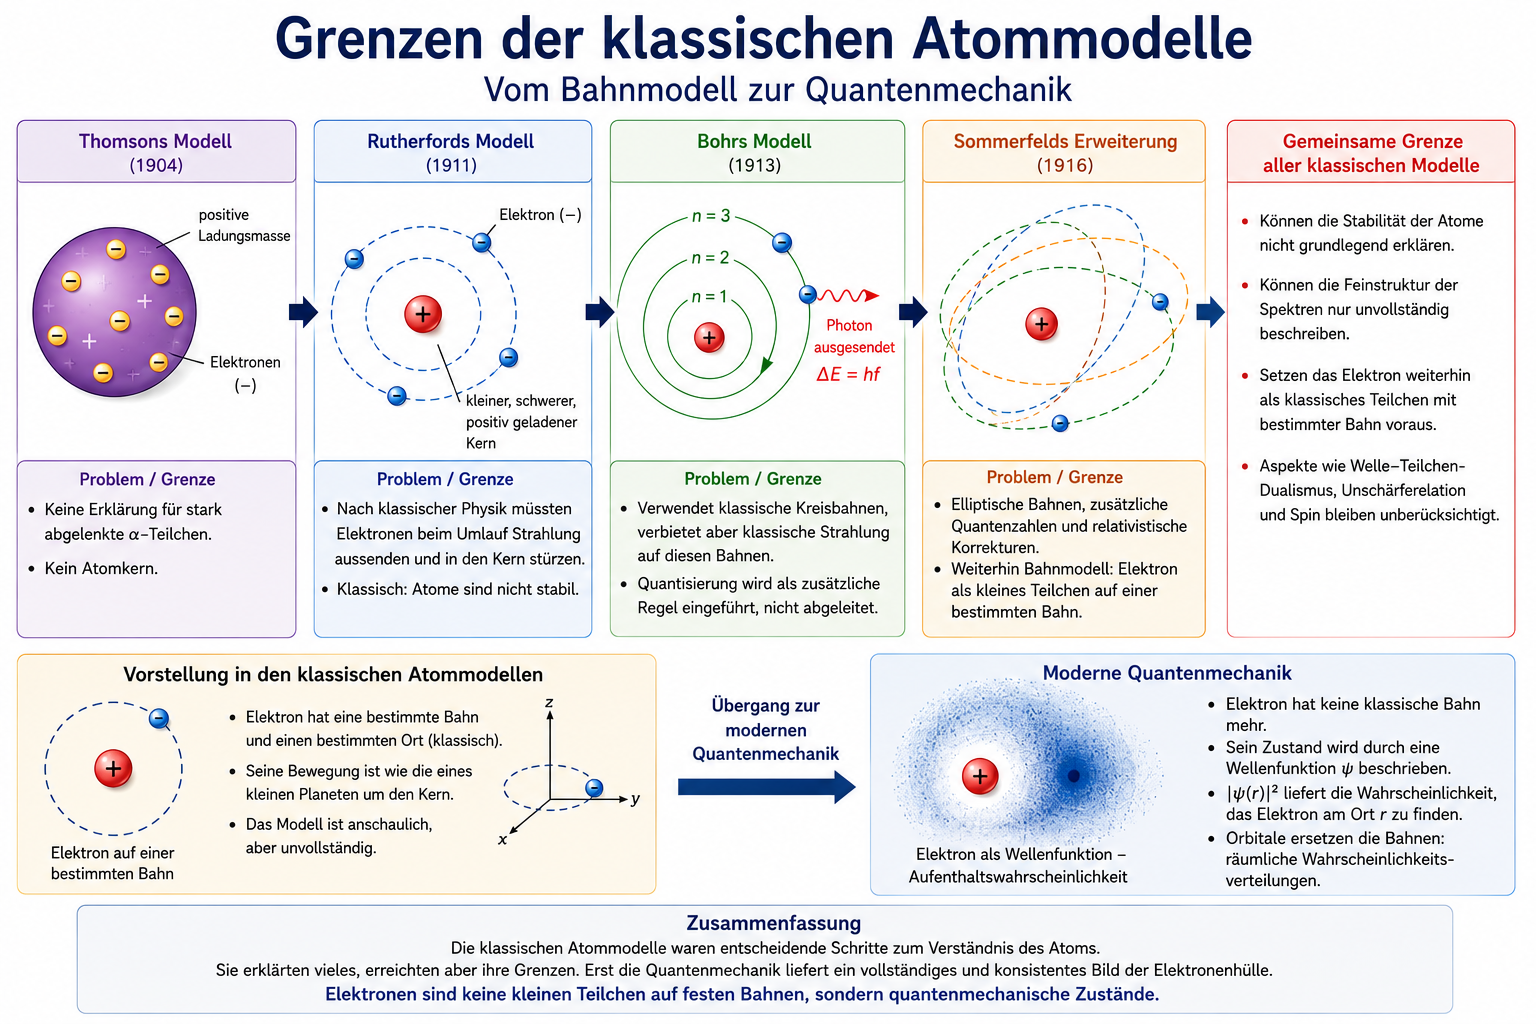
\includegraphics[width=0.78\textwidth]{bilder/grenzen_klassisches_atommodell}
	\caption{Übergang von klassischen Atommodellen zur modernen
		Quantenmechanik. Die Vorstellung fester Elektronenbahnen wird durch
		Wellenfunktionen und Aufenthaltswahrscheinlichkeiten ersetzt.}
	\label{fig:grenzen_klassischer_atommodelle}
\end{figure}

Die Grenzen der klassischen Atommodelle lassen sich daher in drei Punkten
zusammenfassen:

\begin{enumerate}
	\item Klassische Bahnmodelle können die Stabilität der Atome nicht
	grundlegend erklären.
	
	\item Die Spektrallinien der Atome zeigen, dass Energiezustände diskret
	sind und nicht kontinuierlich beliebige Werte annehmen.
	
	\item Der Zustand eines Elektrons im Atom wird nicht durch eine klassische
	Bahn beschrieben, sondern durch quantenmechanische Zustände.
\end{enumerate}

Damit führen die klassischen Atommodelle direkt zur Quantenmechanik. Sie waren
nicht einfach falsch, sondern unvollständig. Sie beschrieben bestimmte
experimentelle Befunde erstaunlich gut, aber sie konnten nicht erklären, warum
die Natur sich auf atomarer Ebene so verhält.

Für das Elektron ist dieser Übergang entscheidend. In den frühen Atommodellen
war es zunächst ein eingebettetes Teilchen, dann ein Teilchen in einer Hülle,
später ein Teilchen auf quantisierten Bahnen. In der Quantenmechanik wird es
schließlich als quantenmechanisches Objekt verstanden, dessen Verhalten nicht
mehr mit den Bildern der klassischen Mechanik beschrieben werden kann.

\begin{DidacticBox}[Die entscheidende Grenze]
	
	\label{box:grenze-klassische-atommodelle}
	Die klassischen Atommodelle benutzen noch das Bild eines Elektrons auf einer
	bestimmten Bahn. Genau diese Vorstellung wird in der modernen Quantenmechanik
	aufgegeben.
	
	Ein Elektron im Atom besitzt keine klassische Bahn mehr. Sein Zustand wird
	durch eine Wellenfunktion beschrieben. Aus ihr ergeben sich
	Aufenthaltswahrscheinlichkeiten, aber keine festen Planetenbahnen.
	
\end{DidacticBox}